\PassOptionsToPackage{unicode=true}{hyperref} % options for packages loaded elsewhere
\PassOptionsToPackage{hyphens}{url}
%
\documentclass[]{article}
\usepackage{lmodern}
\usepackage{setspace}
\setstretch{1}
\usepackage{amssymb,amsmath}
\usepackage{ifxetex,ifluatex}
\usepackage{fixltx2e} % provides \textsubscript
\ifnum 0\ifxetex 1\fi\ifluatex 1\fi=0 % if pdftex
  \usepackage[T1]{fontenc}
  \usepackage[utf8]{inputenc}
  \usepackage{textcomp} % provides euro and other symbols
\else % if luatex or xelatex
  \usepackage{unicode-math}
  \defaultfontfeatures{Ligatures=TeX,Scale=MatchLowercase}
\fi
% use upquote if available, for straight quotes in verbatim environments
\IfFileExists{upquote.sty}{\usepackage{upquote}}{}
% use microtype if available
\IfFileExists{microtype.sty}{%
\usepackage[]{microtype}
\UseMicrotypeSet[protrusion]{basicmath} % disable protrusion for tt fonts
}{}
\IfFileExists{parskip.sty}{%
\usepackage{parskip}
}{% else
\setlength{\parindent}{0pt}
\setlength{\parskip}{6pt plus 2pt minus 1pt}
}
\usepackage{hyperref}
\hypersetup{
            pdftitle={markdown},
            pdfauthor={Gustavo Jun Yakushiji},
            pdfborder={0 0 0},
            breaklinks=true}
\urlstyle{same}  % don't use monospace font for urls
\usepackage[left=3cm, right=3cm, top=2.5cm, bottom=2.5cm]{geometry}
\usepackage{color}
\usepackage{fancyvrb}
\newcommand{\VerbBar}{|}
\newcommand{\VERB}{\Verb[commandchars=\\\{\}]}
\DefineVerbatimEnvironment{Highlighting}{Verbatim}{commandchars=\\\{\}}
% Add ',fontsize=\small' for more characters per line
\usepackage{framed}
\definecolor{shadecolor}{RGB}{42,33,28}
\newenvironment{Shaded}{\begin{snugshade}}{\end{snugshade}}
\newcommand{\AlertTok}[1]{\textcolor[rgb]{1.00,1.00,0.00}{#1}}
\newcommand{\AnnotationTok}[1]{\textcolor[rgb]{0.00,0.40,1.00}{\textbf{\textit{#1}}}}
\newcommand{\AttributeTok}[1]{\textcolor[rgb]{0.74,0.68,0.62}{#1}}
\newcommand{\BaseNTok}[1]{\textcolor[rgb]{0.27,0.67,0.26}{#1}}
\newcommand{\BuiltInTok}[1]{\textcolor[rgb]{0.74,0.68,0.62}{#1}}
\newcommand{\CharTok}[1]{\textcolor[rgb]{0.02,0.61,0.04}{#1}}
\newcommand{\CommentTok}[1]{\textcolor[rgb]{0.00,0.40,1.00}{\textbf{\textit{#1}}}}
\newcommand{\CommentVarTok}[1]{\textcolor[rgb]{0.74,0.68,0.62}{#1}}
\newcommand{\ConstantTok}[1]{\textcolor[rgb]{0.74,0.68,0.62}{#1}}
\newcommand{\ControlFlowTok}[1]{\textcolor[rgb]{0.26,0.66,0.93}{\textbf{#1}}}
\newcommand{\DataTypeTok}[1]{\textcolor[rgb]{0.74,0.68,0.62}{\underline{#1}}}
\newcommand{\DecValTok}[1]{\textcolor[rgb]{0.27,0.67,0.26}{#1}}
\newcommand{\DocumentationTok}[1]{\textcolor[rgb]{0.00,0.40,1.00}{\textit{#1}}}
\newcommand{\ErrorTok}[1]{\textcolor[rgb]{1.00,1.00,0.00}{\textbf{#1}}}
\newcommand{\ExtensionTok}[1]{\textcolor[rgb]{0.74,0.68,0.62}{#1}}
\newcommand{\FloatTok}[1]{\textcolor[rgb]{0.27,0.67,0.26}{#1}}
\newcommand{\FunctionTok}[1]{\textcolor[rgb]{1.00,0.58,0.35}{\textbf{#1}}}
\newcommand{\ImportTok}[1]{\textcolor[rgb]{0.74,0.68,0.62}{#1}}
\newcommand{\InformationTok}[1]{\textcolor[rgb]{0.00,0.40,1.00}{\textbf{\textit{#1}}}}
\newcommand{\KeywordTok}[1]{\textcolor[rgb]{0.26,0.66,0.93}{\textbf{#1}}}
\newcommand{\NormalTok}[1]{\textcolor[rgb]{0.74,0.68,0.62}{#1}}
\newcommand{\OperatorTok}[1]{\textcolor[rgb]{0.74,0.68,0.62}{#1}}
\newcommand{\OtherTok}[1]{\textcolor[rgb]{0.74,0.68,0.62}{#1}}
\newcommand{\PreprocessorTok}[1]{\textcolor[rgb]{0.74,0.68,0.62}{\textbf{#1}}}
\newcommand{\RegionMarkerTok}[1]{\textcolor[rgb]{0.74,0.68,0.62}{#1}}
\newcommand{\SpecialCharTok}[1]{\textcolor[rgb]{0.02,0.61,0.04}{#1}}
\newcommand{\SpecialStringTok}[1]{\textcolor[rgb]{0.02,0.61,0.04}{#1}}
\newcommand{\StringTok}[1]{\textcolor[rgb]{0.02,0.61,0.04}{#1}}
\newcommand{\VariableTok}[1]{\textcolor[rgb]{0.74,0.68,0.62}{#1}}
\newcommand{\VerbatimStringTok}[1]{\textcolor[rgb]{0.02,0.61,0.04}{#1}}
\newcommand{\WarningTok}[1]{\textcolor[rgb]{1.00,1.00,0.00}{\textbf{#1}}}
\usepackage{longtable,booktabs}
% Fix footnotes in tables (requires footnote package)
\IfFileExists{footnote.sty}{\usepackage{footnote}\makesavenoteenv{longtable}}{}
\usepackage{graphicx,grffile}
\makeatletter
\def\maxwidth{\ifdim\Gin@nat@width>\linewidth\linewidth\else\Gin@nat@width\fi}
\def\maxheight{\ifdim\Gin@nat@height>\textheight\textheight\else\Gin@nat@height\fi}
\makeatother
% Scale images if necessary, so that they will not overflow the page
% margins by default, and it is still possible to overwrite the defaults
% using explicit options in \includegraphics[width, height, ...]{}
\setkeys{Gin}{width=\maxwidth,height=\maxheight,keepaspectratio}
\setlength{\emergencystretch}{3em}  % prevent overfull lines
\providecommand{\tightlist}{%
  \setlength{\itemsep}{0pt}\setlength{\parskip}{0pt}}
\setcounter{secnumdepth}{5}
% Redefines (sub)paragraphs to behave more like sections
\ifx\paragraph\undefined\else
\let\oldparagraph\paragraph
\renewcommand{\paragraph}[1]{\oldparagraph{#1}\mbox{}}
\fi
\ifx\subparagraph\undefined\else
\let\oldsubparagraph\subparagraph
\renewcommand{\subparagraph}[1]{\oldsubparagraph{#1}\mbox{}}
\fi

% set default figure placement to htbp
\makeatletter
\def\fps@figure{htbp}
\makeatother

\usepackage[portuguese]{babel}

\title{markdown}
\author{Gustavo Jun Yakushiji}
\date{}

\begin{document}
\maketitle

{
\setcounter{tocdepth}{2}
\tableofcontents
}
\hypertarget{titulo}{%
\section{Titulo}\label{titulo}}

No penúltimo jogo da Copa América de 2020, a Colômbia venceu o Peru de
virada por 3 a 2 em Brasília nesta sexta-feira e ficou com o terceiro
lugar na classificação geral da competição.

O Peru abriu o placar aos 45 minutos do primeiro tempo com Yotun. Na
etapa final, a Colômbia virou com Cuadrado aos 4 minutos e Luis Diáz aos
21 da etapa final. Aos 37 do segundo tempo, Lapadula, de cabeça, empatou
o confronto para os peruanos.

\hypertarget{titulo-1}{%
\subsection{Titulo}\label{titulo-1}}

No penúltimo jogo da Copa América de 2020, a Colômbia venceu o Peru de
virada por 3 a 2 em Brasília nesta sexta-feira e ficou com o terceiro
lugar na classificação geral da competição.

O Peru abriu o placar aos 45 minutos do primeiro tempo com Yotun. Na
etapa final, a Colômbia virou com Cuadrado aos 4 minutos e Luis Diáz aos
21 da etapa final. Aos 37 do segundo tempo, Lapadula, de cabeça, empatou
o confronto para os peruanos.

\hypertarget{titulo-2}{%
\subsubsection{Titulo}\label{titulo-2}}

No penúltimo jogo da Copa América de 2020, a Colômbia venceu o Peru de
virada por 3 a 2 em Brasília nesta sexta-feira e ficou com o terceiro
lugar na classificação geral da competição.

O Peru abriu o placar aos 45 minutos do primeiro tempo com Yotun. Na
etapa final, a Colômbia virou com Cuadrado aos 4 minutos e Luis Diáz aos
21 da etapa final. Aos 37 do segundo tempo, Lapadula, de cabeça, empatou
o confronto para os peruanos.

\begin{Shaded}
\begin{Highlighting}[]
\KeywordTok{summary}\NormalTok{(pressure)}
\end{Highlighting}
\end{Shaded}

\begin{verbatim}
##   temperature     pressure       
##  Min.   :  0   Min.   :  0.0002  
##  1st Qu.: 90   1st Qu.:  0.1800  
##  Median :180   Median :  8.8000  
##  Mean   :180   Mean   :124.3367  
##  3rd Qu.:270   3rd Qu.:126.5000  
##  Max.   :360   Max.   :806.0000
\end{verbatim}

\begin{figure}

{\centering 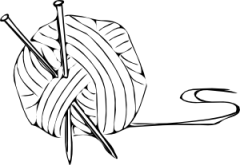
\includegraphics[width=3.33in]{knit_logo} 

}

\caption{Knitr logo}\label{fig:unnamed-chunk-2}
\end{figure}

\hypertarget{fuxf3rmulas}{%
\subsection{Fórmulas}\label{fuxf3rmulas}}

Veja \(f(x)=x^2\)

A seguir um gráfico de dispersão dos nossos dados\ldots{}(Veja Figura
\ref{scatterplot})

\begin{Shaded}
\begin{Highlighting}[]
\KeywordTok{plot}\NormalTok{(Ozone}\OperatorTok{~}\NormalTok{Wind, }\DataTypeTok{data=}\NormalTok{airquality, }\DataTypeTok{pch=}\DecValTok{20}\NormalTok{, }
     \DataTypeTok{col=}\StringTok{"darkorange"}\NormalTok{, }\DataTypeTok{lwd=}\DecValTok{3}\NormalTok{)}
\end{Highlighting}
\end{Shaded}

\begin{figure}
\centering
\includegraphics{Iniciando_markdown_Gustavo_files/figure-latex/unnamed-chunk-3-1.pdf}
\caption{\label{scatterplot}Titulo do meu gráfico}
\end{figure}

A seguir o ajuste do modelo usando o \textcolor{red}{software R}

\begin{Shaded}
\begin{Highlighting}[]
\NormalTok{ajuste<-}\StringTok{ }\KeywordTok{lm}\NormalTok{(Ozone}\OperatorTok{~}\NormalTok{Wind, }\DataTypeTok{data=}\NormalTok{airquality)}
\NormalTok{teta<-}\StringTok{ }\KeywordTok{round}\NormalTok{(}\KeywordTok{coef}\NormalTok{(ajuste),}\DecValTok{3}\NormalTok{)}
\NormalTok{betaS<-}\StringTok{ }\KeywordTok{round}\NormalTok{(}\KeywordTok{coef}\NormalTok{(}\KeywordTok{summary}\NormalTok{(ajuste)),}\DecValTok{3}\NormalTok{)}
\NormalTok{knitr}\OperatorTok{::}\KeywordTok{kable}\NormalTok{(betaS, }\DataTypeTok{caption =} \StringTok{"}\CharTok{\textbackslash{}\textbackslash{}}\StringTok{label\{tabelajuste\}}
\StringTok{             Ajuste de um ML para os dados airquality"}\NormalTok{)}
\end{Highlighting}
\end{Shaded}

\begin{longtable}[]{@{}lrrrr@{}}
\caption{\label{tabelajuste} Ajuste de um ML para os dados
airquality}\tabularnewline
\toprule
& Estimate & Std. Error & t value &
Pr(\textgreater{}\textbar{}t\textbar{})\tabularnewline
\midrule
\endfirsthead
\toprule
& Estimate & Std. Error & t value &
Pr(\textgreater{}\textbar{}t\textbar{})\tabularnewline
\midrule
\endhead
(Intercept) & 96.873 & 7.239 & 13.383 & 0\tabularnewline
Wind & -5.551 & 0.690 & -8.040 & 0\tabularnewline
\bottomrule
\end{longtable}

O modelo ajustado foi \(\widehat{\text{Ozone}}_i=\) 96.873 -5.551
\(\text{Wind}_i\) (Veja Tabela \ref{tabelajuste})

\begin{Shaded}
\begin{Highlighting}[]
\KeywordTok{citation}\NormalTok{(}\StringTok{"ggplot2"}\NormalTok{)}
\end{Highlighting}
\end{Shaded}

\begin{verbatim}
## 
## To cite ggplot2 in publications, please use:
## 
##   H. Wickham. ggplot2: Elegant Graphics for Data Analysis.
##   Springer-Verlag New York, 2016.
## 
## A BibTeX entry for LaTeX users is
## 
##   @Book{,
##     author = {Hadley Wickham},
##     title = {ggplot2: Elegant Graphics for Data Analysis},
##     publisher = {Springer-Verlag New York},
##     year = {2016},
##     isbn = {978-3-319-24277-4},
##     url = {https://ggplot2.tidyverse.org},
##   }
\end{verbatim}

\begin{Shaded}
\begin{Highlighting}[]
\KeywordTok{library}\NormalTok{(ggplot2)}
\end{Highlighting}
\end{Shaded}

Podemos usar Wickham (2016) ou (Wickham 2016).

\hypertarget{referuxeancias}{%
\section*{Referências}\label{referuxeancias}}
\addcontentsline{toc}{section}{Referências}

\hypertarget{refs}{}
\leavevmode\hypertarget{ref-ggplot2}{}%
Wickham, Hadley. 2016. \emph{Ggplot2: Elegant Graphics for Data
Analysis}. Springer-Verlag New York. \url{http://ggplot2.org}.

\end{document}
